\section{{Descripción casos de uso}}

%--------------------------Inicia otro caso de uso (javier)--------------------------------------------------------------%

\subsection{\textcolor{blue}{CU 1.1 Restablecer contraseña}}

\subsubsection{\textcolor{blue}{Resumen}}
Se brindara al usuario la posibilidad de recuperar sus datos para acceder al sistenma en caso de haberlos olvidado o perdido.
\subsubsection{\textcolor{blue}{Descripción}}
\begin{tabularx}{16cm}{||l|X||}
	\hline
	\multicolumn{2}{||c||}{Caso de Uso: Reestablecer contraseña } \\
	\hline
	\multicolumn{2}{||c||}{\textcolor{blue}{Resumen de atributos}} \\
	\hline
	{Autor:} & Zamarrón Ramírez Javier \\
    \hline
	{Actor:} & Usuario turista\\
	\hline
	{Próposito:} & Permitir al usuario restablecer contraseña\\
	\hline
	{Entradas:} &  Se escribe desde la pantalla del celular el correo electrónico del usuario. \\
	\hline
	{Salidas:} & Se envía el mensaje de correo electrónico de recuperación de contraseña \\
	\hline
	{Precondiciones:} & Debe existir una cuenta activa en el sistema con el correo electronico.\\ 
	\hline
	{Postcondiciones:} & Se elimina la cuenta del usuario, por lo que el sistema deja de almacenar su informacion.\\
	\hline
	{Errores:} &\begin{minipage}{1\linewidth}
        \begin{enumerate}
            \item Cuando el correo electrónico no es válido, se mostrará el mensaje de alerta 1.
            \item Cuando el correo electrónico no está asociado a una cuenta activa, se mostrará el mensaje de alerta 2.
            \item Cuando las contraseñas no son iguales, se mostrará el mensaje de alerta 3.
            \item Cuando la contraseña no cumple con la regla de negocio 5, se mostrará el mensaje de alerta 4.
        \end{enumerate}
    \end{minipage} \\
	\hline
	{Tipo:} & Reunion interna\\
	\hline
	{Fuente:} & {-} \\
	\hline
	{Observaciones:} & {-} \\
	\hline
\end{tabularx}

\pagebreak
\subsubsection{\textcolor{blue}{Trayectorias del caso de uso}}
\textbf{Trayectoria Principal}
    \begin{enumerate}
    \item 
\includegraphics[width=0.0150\textwidth]{Figuras/persona.png} presiona la leyenda olvidaste tu contraseña? en la pantalla \textcolor{blue}{Iniciar sesion}.
    \item 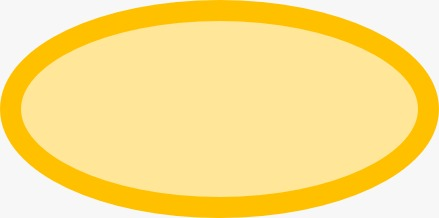
\includegraphics[width=0.0500\textwidth]{Figuras/sistema.png} muestra la pantalla Recuperar contraseña.
    \item 
\includegraphics[width=0.0150\textwidth]{Figuras/persona.png} solicita recuperar los datos de su cuenta oprimiendo ¿Olvidaste tu contraseña? de la pantalla \textcolor{blue}{Iniciar sesion}.
     \item 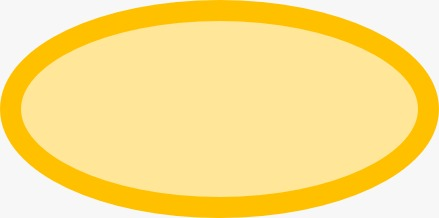
\includegraphics[width=0.0500\textwidth]{Figuras/sistema.png} solicita ingresar el correo electronico asociado a la cuenta de la que se desea reestablecer la contraseña mostrando la pantalla \textcolor{blue}{Recuperacion de contraseña} [Trayectoria A].
    \item 
\includegraphics[width=0.0150\textwidth]{Figuras/persona.png} ingresa el correo electronico .
    \item 
\includegraphics[width=0.0150\textwidth]{Figuras/persona.png} solicita reestablecer la contraseña de su cuenta oprimiendo el boton de enviar correo.
    \item 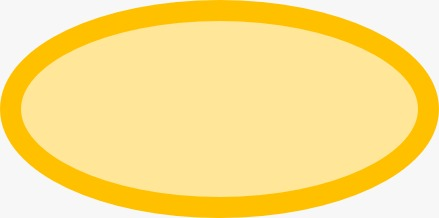
\includegraphics[width=0.0500\textwidth]{Figuras/sistema.png} verifica que el correo electronico sea valido. [Trayectoria B]
    \item 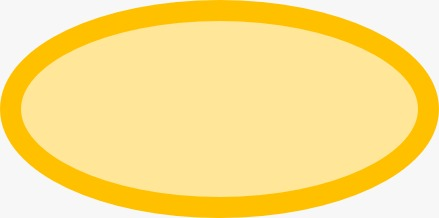
\includegraphics[width=0.0500\textwidth]{Figuras/sistema.png} verifica que el correo electronico este asociado a una cuenta activa. [Trayectoria C].
    \item 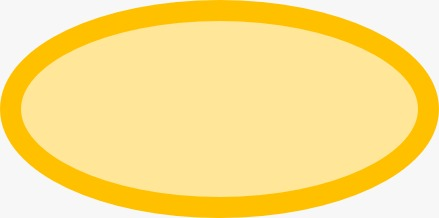
\includegraphics[width=0.0500\textwidth]{Figuras/sistema.png} genera y registra el token de restablecimiento de contraseña.
    \item 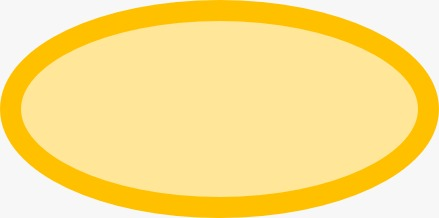
\includegraphics[width=0.0500\textwidth]{Figuras/sistema.png} envia por correo electronico el mensaje \textcolor{blue}{E-mail1 Correo recuperación de contraseña} .
    \item 
\includegraphics[width=0.0150\textwidth]{Figuras/persona.png} accede al enlace enviado por correo electrónico.
    \item 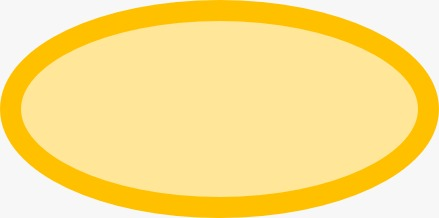
\includegraphics[width=0.0500\textwidth]{Figuras/sistema.png} recibe la solicitud del usuario para restablecer contraseña.
    \item 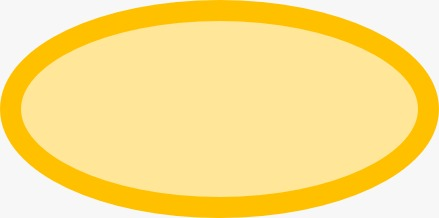
\includegraphics[width=0.0500\textwidth]{Figuras/sistema.png} verifica que el token de la cuenta sea valido.
    \item 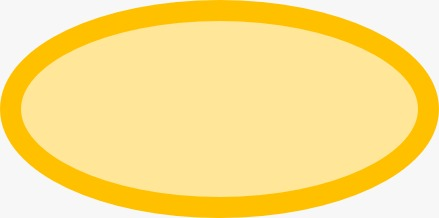
\includegraphics[width=0.0500\textwidth]{Figuras/sistema.png} verifica que el token de la cuenta sea valido.
    \item 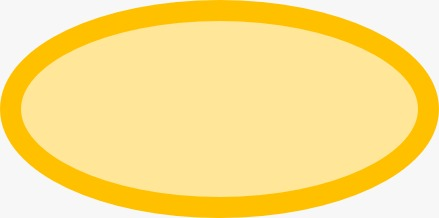
\includegraphics[width=0.0500\textwidth]{Figuras/sistema.png} muestra al usuario la pantalla de Restablecer contraseña.
    \item 
\includegraphics[width=0.0150\textwidth]{Figuras/persona.png} escribe sus contraseñas y presiona el boton Guardar contraseña.
    \item 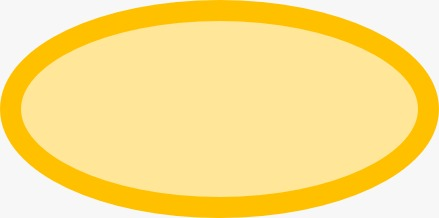
\includegraphics[width=0.0500\textwidth]{Figuras/sistema.png} verifica si ambas contraseñas son iguales. [Trayectoria D]
    \item 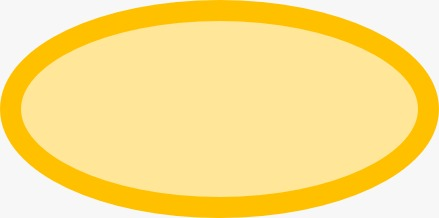
\includegraphics[width=0.0500\textwidth]{Figuras/sistema.png} verifica si la contraseña proporcionada cumple con los requisitos mencionados en la regla de negocio 5. [Trayectoria E]
    \item 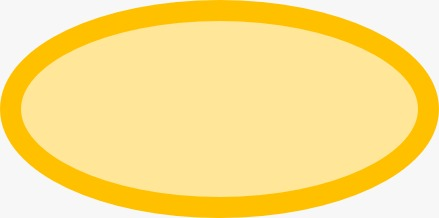
\includegraphics[width=0.0500\textwidth]{Figuras/sistema.png} elimina el token de restablecimiento de contraseña generado.
    \item 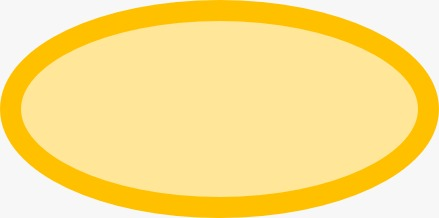
\includegraphics[width=0.0500\textwidth]{Figuras/sistema.png} actualiza la contraseña del usuario.
    \item 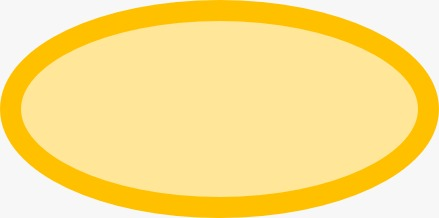
\includegraphics[width=0.0500\textwidth]{Figuras/sistema.png} muestra la pantalla Recuperacion de contraseña (exitoso) y se redirecciona a pantalla Iniciar sesion.\\
    - - - Fin de caso de uso
\end{enumerate}

\textbf{Trayectoria A}\\
Condición : 
\includegraphics[width=0.0150\textwidth]{Figuras/persona.png} desea cancelar el cambio de contraseña
\begin{itemize}
    \item 
\includegraphics[width=0.0150\textwidth]{Figuras/persona.png} oprime el boton de regresar.
     \item 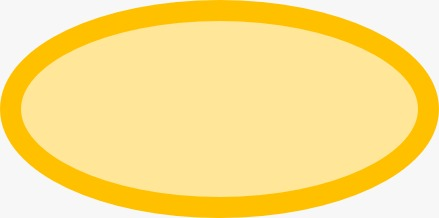
\includegraphics[width=0.0500\textwidth]{Figuras/sistema.png} muestra la pantalla Iniciar sesion.
    \item Termina el caso de uso.\\
    - - - Fin de trayectoria
\end{itemize}
\textbf{Trayectoria B}\\
Condición :  
\includegraphics[width=0.0150\textwidth]{Figuras/persona.png} no escribio un correo valido.
\begin{itemize}
    \item 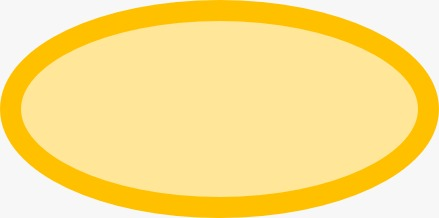
\includegraphics[width=0.0500\textwidth]{Figuras/sistema.png} muestra en la pantalla Recuperacion de contraseña el mensaje alerta 1.
    \item Continua en el paso 5\\
    - - - Fin de trayectoria
\end{itemize}
\textbf{Trayectoria C}\\
Condición : 
\includegraphics[width=0.0150\textwidth]{Figuras/persona.png} escribio un correo electronico que no esta asociado a una cuenta activa.
\begin{itemize}
    \item 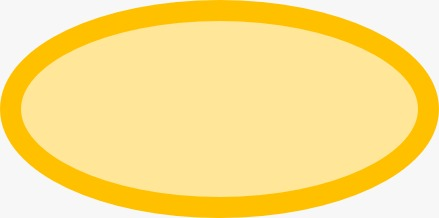
\includegraphics[width=0.0500\textwidth]{Figuras/sistema.png} muestra en la pantalla Recuperacion de contraseña el mensaje alerta 2.
    \item Continua en el paso 3\\
    - - - Fin de trayectoria
\end{itemize}
\textbf{Trayectoria D}\\
Condición : Las contraseñas escritas por 
\includegraphics[width=0.0150\textwidth]{Figuras/persona.png} no son iguales.
\begin{itemize}
    \item  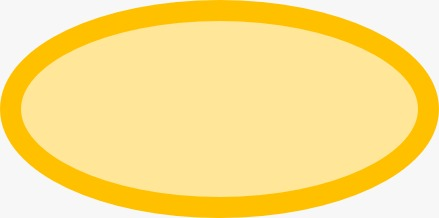
\includegraphics[width=0.0500\textwidth]{Figuras/sistema.png} muestra en la pantalla restablecer contraseña el mensaje alerta 3.
    \item Continua en el paso 14.\\
    - - - Fin de trayectoria
\end{itemize}
\textbf{Trayectoria E}\\
Condición : La contraseña escrita por el 
\includegraphics[width=0.0150\textwidth]{Figuras/persona.png} no cumple con la regla de negocio 5.
\begin{itemize}
    \item 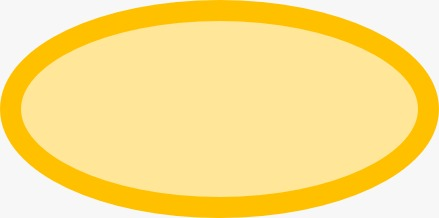
\includegraphics[width=0.0500\textwidth]{Figuras/sistema.png} muestra en la pantalla restablecer contraseña el mensaje alerta 4.
    \item Continua en el paso 14.\\
    - - - Fin de trayectoria
\end{itemize}
\subsubsection{\textcolor{blue}{Pantalla IU3 y IU4}}

    \begin{figure}[htb]
        \centering
        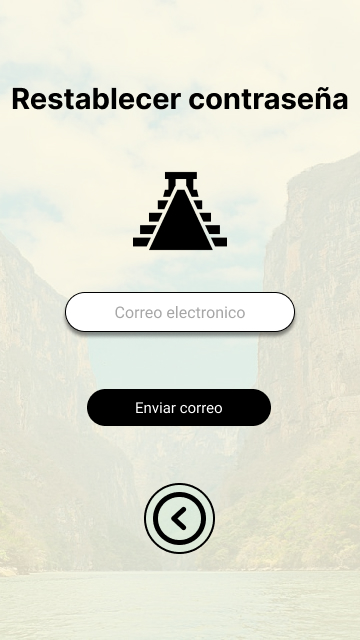
\includegraphics[width= 5cm]{Pantallas Prototipo3/IU03 Pantalla correo restablecimiento.jpg}
        \caption{IU03 Recuprar contraseña}
        \label{fig:enter-label}
    \end{figure}
    \begin{figure}[htb]
        \centering
        \includegraphics[width= 5cm]{Pantallas Prototipo3/IU05-Reestablacer contraseña.jpg}
        \caption{IU04 Escribir contraseña nueva}
        \label{fig:enter-label}
    \end{figure}

%---------------------------------------Finaliza caso de uso (javier)%---------------------------------------------------
%-----------------------------------------------------------------------------------------------------------------------

















%--------------------------Inicia otro caso de uso (said)--------------------------------------------------------------%

\subsection{\textcolor{blue}{CU 2.2 Eliminar cuenta}}

\subsubsection{\textcolor{blue}{Resumen}}
Se brinda al usuario la posibilidad de poder eliminar su cuenta, además se necesita ingresar la contraseña como metodo de validacion.
\subsubsection{\textcolor{blue}{Descripción}}
\begin{tabularx}{16cm}{||l|X||}
	\hline
	\multicolumn{2}{||c||}{Caso de Uso: } \\
	\hline
	\multicolumn{2}{||c||}{\textcolor{blue}{Resumen de atributos}} \\
	\hline
	{Autor:} & Estrada Yepez Omar Said \\
    \hline
	{Actor:} & Usuario turista\\
	\hline
	{Próposito:} & Que el sistema permita al usuario eliminar su cuenta en cualquier momento si asi lo desea.\\
	\hline
	{Entradas:} &  Boton con el nombre de Actualizar datos. \\
    &Se ingresa la contraseña del usuario\\
    &Se ingresa la confirmacion de la contraseña del usuario.\\
    &Boton para validar contraseñas\\
    &Boton de confirmacion de eliminar\\
	\hline
	{Salidas:} & En la pantalla se mostrara el mensaje "Su cuenta fue eliminada con exito"\\
	\hline
	{Precondiciones:} & Debe existir una cuenta activa en el sistema con el correo electronico.\\ 
	\hline
	{Postcondiciones:} & Se elimina la cuenta del usuario, por lo que el sistema deja de almacenar su informacion.\\
	\hline
	{Errores:} & Cuando se proporciona la contraseña no coincide con el formato requerido de una contraseña. \\
    &No coincide la contraseña con la confirmacion de contraseña, se muestra el mensaje Las contraseñas deben ser iguales.\\
	\hline
	{Tipo:} & -\\
	\hline
	{Fuente:} & Reunion interna \\
	\hline
	{Observaciones:} & {-} \\
	\hline
\end{tabularx}

\pagebreak
\subsubsection{\textcolor{blue}{Trayectorias del caso de uso}}
\textbf{Trayectoria Principal}
    \begin{enumerate}
        \item 
\includegraphics[width=0.0150\textwidth]{Figuras/persona.png} El usuario solicita modificar datos oprimiendo el boton 
\includegraphics[width=0.2\textwidth]{ComponentesCU/AD.png}  de la Pantalla de perfil.
        \item 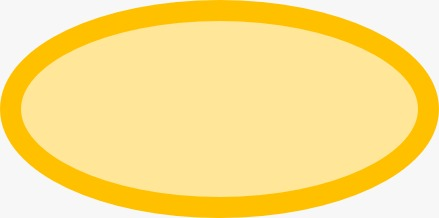
\includegraphics[width=0.0500\textwidth]{Figuras/sistema.png} Muestra la Pantalla de seleccionar el dato a editar, mostrando en la parte inferior derecha el boton 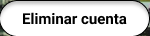
\includegraphics[width=0.2\textwidth]{ComponentesCU/img.png}.
        \item 
\includegraphics[width=0.0150\textwidth]{Figuras/persona.png} Oprime el boton 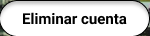
\includegraphics[width=0.2\textwidth]{ComponentesCU/img.png}.
         \item 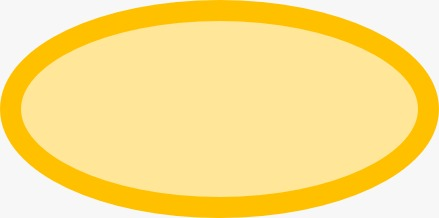
\includegraphics[width=0.0500\textwidth]{Figuras/sistema.png} Muestra la pantalla Validacion de contraseña para modificacion de datos.
        \item 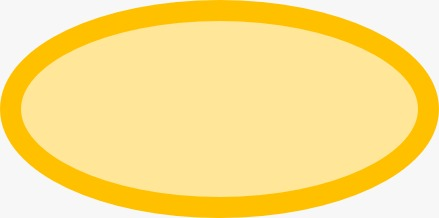
\includegraphics[width=0.0500\textwidth]{Figuras/sistema.png} Solicita la contraseña y confirmacion de contraseña del usuario.
        \item 
\includegraphics[width=0.0150\textwidth]{Figuras/persona.png} Ingresa su contraseña y su confirmacion de la misma.
        \item 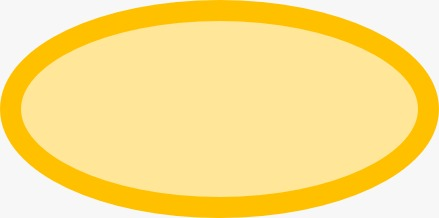
\includegraphics[width=0.0500\textwidth]{Figuras/sistema.png} Valida que las contraseñas sean iguales[Trayectoria A].
        \item 
\includegraphics[width=0.0150\textwidth]{Figuras/persona.png} Oprime el boton 
\includegraphics[width=0.2\textwidth]{ComponentesCU/img1.png} de la pantalla Validacion de contraseña para modificacion de datos.
        \item 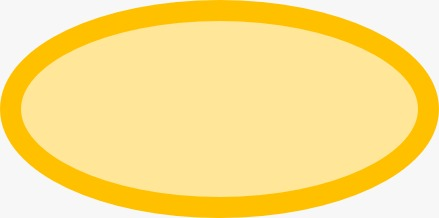
\includegraphics[width=0.0500\textwidth]{Figuras/sistema.png} Muestra la pantalla Ventana de confirmación de eliminar cuenta con el mensaje ¿Estas seguro de eliminar tu cuenta?
        \item 
\includegraphics[width=0.0150\textwidth]{Figuras/persona.png} Oprime el boton 
\includegraphics[width=0.25\textwidth]{ComponentesCU/img2.png} [Trayectoria B].
        \item 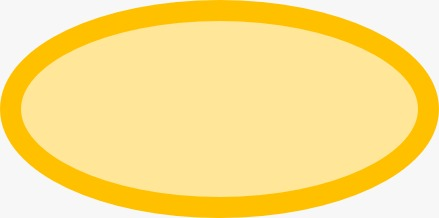
\includegraphics[width=0.0500\textwidth]{Figuras/sistema.png} Elimina el perfil del usuario turista.
        \item \includegraphics[width=0.0500\textwidth]{Figuras/sistema.png} Muestra el mensaje Su cuenta fue eliminada con exito
    \end{enumerate}
---FIN DE LA TRAYECTORIA--\\\\
\textbf{Trayectoria A}
    \begin{enumerate}
        \item \includegraphics[width=0.0500\textwidth]{Figuras/sistema.png} Muestra en la pantalla Validacion de contraseña erronea para modificacion de datos el mensaje Las contraseñas deben ser iguales indicando al usuario que las contraseñas son diferentes.
        \item \includegraphics[width=0.0500\textwidth]{Figuras/sistema.png} Continua el paso 5 de la trayectoria principal.
    \end{enumerate}
---FIN DE LA TRAYECTORIA--\\\\
\textbf{Trayectoria B}
    \begin{enumerate}
        \item \includegraphics[width=0.0150\textwidth]{Figuras/persona.png} Oprime el boton \includegraphics[width=0.25\textwidth]{ComponentesCU/img3.png}
        \item \includegraphics[width=0.0500\textwidth]{Figuras/sistema.png} Muestra la Pantalla de perfil
    \end{enumerate}
---FIN DE LA TRAYECTORIA--
\newpage
\subsubsection{\textcolor{blue}{Pantalla IUXXX}}
\begin{figure}[htbp]
        \centering
        \includegraphics[width= 5cm]{Pantallas Prototipo3/IU14 Pantalla de perfil.jpg}
        \caption{Pantalla de perfil}
        \label{fig:enter-label}
\end{figure}
\begin{figure}[htbp]
    \centering
    \includegraphics[width= 5cm]{Pantallas Prototipo3/IU16 Pantalla de seleccionar el dato a editar.jpg}
    \caption{Pantalla de seleccionar el dato a editar}
    \label{fig:enter-label}
\end{figure}

\begin{figure}[htbp]
        \centering
        \includegraphics[width= 5cm]{Pantallas Prototipo3/IU15 Pantalla Validacion de Contraseña.jpg}
        \caption{Validacion de contraseña para modificacion de datos}
        \label{fig:enter-label}
\end{figure}

\begin{figure}[htbp]
        \centering
        \includegraphics[width= 5cm]{Pantallas Prototipo3/IU19 Pantalla Ventana de confirmación de eliminar cuenta.jpg}
        \caption{Ventana de confirmación de eliminar cuenta}
        \label{fig:enter-label}
        \vspace{200pt}
\end{figure}
\newpage
%---------------------------------------Finaliza caso de uso (Said)%---------------------------------------------------
%-----------------------------------------------------------------------------------------------------------------------

%--------------------------Inicia otro caso de uso (Fer)--------------------------------------------------------------%

\subsection{\textcolor{blue}{CU 3 Llenar formulario de datos}}
\subsubsection{\textcolor{blue}{Resumen}}
             Se permite al Usuario Turista llenar los formularios de datos con información personal, al momento en el que se registre; estos datos son esenciales para crear una cuenta de usuario. La privacidad y la seguridad de estos datos personales son fundamentales, garantizando que se utilizan de manera segura y conforme a las políticas de privacidad. El sistema proporciona una interfaz para el ingreso de los datos como el nombre, apellido, correo electrónico, número de teléfono, fecha de nacimiento y contraseña.
             
\subsubsection{Descripción} \\
            \begin{tabularx}{16cm}{||l|X||}
            	\hline
            	\multicolumn{2}{||c||}{Caso de Uso: : Llenar formulario de datos} \\
            	\hline
            	\multicolumn{2}{||c||}{\textcolor{blue}{Resumen de atributos}} \\
            	\hline
            	{Actor:} & {\textcolor{blue}{Usuario Turista}} \\
                \hline
                {Autor:} & {Murillo Mendoza María Fernanda} \\
            	\hline
            	{Próposito:} & {Permite al Usuario Turista llenar formularios de datos con su información personal, al momento en el que se registre.} \\
            	\hline
                 {Entradas:} & { \begin{itemize}
                        \item \textbf Se escribe desde el teclado un usuario válido
                        \item \textbf Se escribe desde el teclado un nombre y un apellido
                        \item \textbf Se escribe desde el teclado un correo electrónico Gmail
                        \item \textbf Se escribe desde el teclado numérico un teléfono móvil 
                        \item \textbf Se escribe desde el teclado una fecha de nacimiento
                        \item \textbf Se escribe desde el teclado una contraseña junto con su confirmación
                        
                    \end{itemize}
                  }\\ 
            	\hline
            	{Salidas:} & {Se mostrará la pantalla \textcolor{blue}{IU06 Pantalla Registro de Cuenta} con el mensaje \textcolor{blue}{MSJ Registro Exitoso} }\\
            	\hline
            	{Precondiciones:} & {Contar con un correo electrónico en Gmail}\\\\
            	\hline
            	{Postcondiciones:} & { 
             \begin{itemize}
                        \item \textbf El usuario podrá acceder al apartado beyamaps.
                        \item \textbf El usuario podrá ver su itinerario.
                        \item \textbf El usuario podrá marcar sus preferencias.
                        \item \textbf El usuario podrá modificar sus datos personales en un futuro.
                        \item \textbf El usuario podrá ver su historial.
                        \item \textbf El usuario podrá agregar y eliminar sus lugares favoritos.
                        \end{itemize}
                } \\
                    \hline
        \end{tabularx}
                  \newpage
                  \begin{tabularx}{16cm}{||l|X||}
                  \hline
            	{Errores:} & { \begin{itemize}
                        \item \textbf Cuando el Usuario Turista no ingresa todos los datos requeridos y hace una omisión.
                        \item \textbf Cuando no coincida la confirmación de contraseña.   
                        \item \textbf Cuando los datos proporcionados por el Usuario Turista no sean verídicos.
                    \end{itemize}
                } \\
            	\hline
            	{Tipo:} & {Secundario para el actor Turista. Viene del caso de uso Registrar Usuario.}\\
            	\hline
            	{Fuente:} & {Reunión Internada de CDT} \\
            	\hline
            	{Observaciones:} & {} \\
            	\hline
            \end{tabularx}  
            
    \subsection{Trayectorias del caso de uso}
     \\
                \begin{enumerate}
                    \item \textbf{Trayectoria principal\\}
                        \item \includegraphics[width=0.0150\textwidth]{Figuras/persona.png}Solicita registrar cuenta oprimiendo el boton "Registrar Cuenta" desde la pantalla \textcolor{blue}{IU01 Pantalla incial}  
                        \item \includegraphics[width=0.0150\textwidth]{Figuras/persona.png} Ingresa desde el teclado un usuario válido 
                        \item \includegraphics[width=0.0500\textwidth]{Figuras/sistema.png} Valida los datos ingresados 
                        [\textcolor{blue}{Trayectoria A}.]
                        [\textcolor{blue}{Trayectoria B}.]
                        
                        \item \includegraphics[width=0.0150\textwidth]{Figuras/persona.png} Ingresa desde el teclado uno o dos nombres
                        \item \includegraphics[width=0.0500\textwidth]{Figuras/sistema.png} Valida los datos ingresados
                        [\textcolor{blue}{Trayectoria C}.]
                        
                        \item \includegraphics[width=0.0150\textwidth]{Figuras/persona.png} Ingresa desde el teclado un apellido 
                       \item \includegraphics[width=0.0500\textwidth]{Figuras/sistema.png} Valida los datos ingresados [\textcolor{blue}{Trayectoria D}.]

                       \item \includegraphics[width=0.0150\textwidth]{Figuras/persona.png} Ingresa desde el teclado un correo en formato Gmail 
                       \item \includegraphics[width=0.0500\textwidth]{Figuras/sistema.png} Valida los datos ingresados [\textcolor{blue}{Trayectoria E}.]

                       \item \includegraphics[width=0.0150\textwidth]{Figuras/persona.png}Ingresa desde el teclado numérico su número de teléfono celular
                       \item \includegraphics[width=0.0500\textwidth]{Figuras/sistema.png} Valida los datos ingresados [\textcolor{blue}{Trayectoria F}.]
                       
                       \item \includegraphics[width=0.0150\textwidth]{Figuras/persona.png} Ingresa desde el teclado una contraseña
                       \item \includegraphics[width=0.0500\textwidth]{Figuras/sistema.png} Valida los datos ingresados [\textcolor{blue}{Trayectoria G}.]

                       \item \includegraphics[width=0.0150\textwidth]{Figuras/persona.png} Ingresa desde el teclado la contraseña anteriormente escrita
                       \item \includegraphics[width=0.0500\textwidth]{Figuras/sistema.png} Valida los datos ingresados [\textcolor{blue}{Trayectoria H}.]

                       \item \includegraphics[width=0.0150\textwidth]{Figuras/persona.png} El usuario da clic en el botón "REGISTRAME"  [\textcolor{blue}{Trayectoria I}.] 
                       \item \includegraphics[width=0.0500\textwidth]{Figuras/sistema.png} Muestra el mensaje \textcolor{blue}{MSJ
Registro Exitoso} en la pantalla \textcolor{blue}{IU06 Pantalla Registro de Cuenta}
                       \item \includegraphics[width=0.0500\textwidth]{Figuras/sistema.png} Envía al usuario a la pantalla \textcolor{blue}{IU07 Preferencias del usuario}

                    \end{enumerate}
                    
                    \textbf{Trayectoria alternativa A:}\\
                        \textbf{Condición:} El nombre de usuario ya está en uso.\\\\
                        \textbf{A1:}\includegraphics[width=0.0500\textwidth]{Figuras/sistema.png} Muestra en la pantalla [\textcolor{blue}{IU06 Pantalla Registro de Cuenta}.] el mensaje de validación [\textcolor{blue}{Usuario existente}.]  \\\\
                        \textbf{A2:}\includegraphics[width=0.0150\textwidth]{Figuras/persona.png}Cambia su nombre de usuario por uno nuevo.\\\\
                        \textbf{A3:}\includegraphics[width=0.0500\textwidth]{Figuras/sistema.png} Valida los datos ingresados\\\\
                        \textbf{A4:}Continúa en el paso 2 \\\\
       
        -------Fin de  trayectoria. \\\\

                    \textbf{Trayectoria alternativa B:}\\
                        \textbf{Condición:}El nombre de usuario no cumple con el formato.\\\\
                        \textbf{A1:}\includegraphics[width=0.0500\textwidth]{Figuras/sistema.png} Muestra en la pantalla [\textcolor{blue}{IU06 Pantalla Registro de Cuenta}.] el mensaje de validación [\textcolor{blue}{El nombre no debe tener espacios}.] y  [\textcolor{blue}{El nombre debe tener un máximo 10 a 15 palabras}.]\\\\ 
                        \textbf{A2:}\includegraphics[width=0.0150\textwidth]{Figuras/persona.png}Modifica su nombre de usuario.\\\\
                        \textbf{A3:}\includegraphics[width=0.0500\textwidth]{Figuras/sistema.png} Valida los datos ingresados\\\\
                        \textbf{A4:}Continúa en el paso 2 \\\\
       
        -------Fin de  trayectoria. \\\\

    
                     \textbf{Trayectoria alternativa C:}\\\\
                        \textbf{Condición:}El nombre no cumple con el formato.\\\\
                        \textbf{A1:}\includegraphics[width=0.0500\textwidth]{Figuras/sistema.png} Muestra en la pantalla [\textcolor{blue}{IU06 Pantalla Registro de Cuenta}.] el mensaje de validación [\textcolor{blue}{No se aceptan números y caracteres especiales (=,*,etc), solamente letras}].  \\\\
                        \textbf{A2:}\includegraphics[width=0.0150\textwidth]{Figuras/persona.png}Cambia su nombre.\\\\
                        \textbf{A3:}\includegraphics[width=0.0500\textwidth]{Figuras/sistema.png} Valida los datos ingresados\\\\
                        \textbf{A4:}Continúa en el paso 4 \\\\
                       
        -------Fin de  trayectoria. \\\\

                    \textbf{Trayectoria alternativa D:}\\
                        \textbf{Condición:}Los apellidos no cumplen con el formato.\\\\
                        \textbf{A1:}\includegraphics[width=0.0500\textwidth]{Figuras/sistema.png} Muestra en la pantalla [\textcolor{blue}{IU06 Pantalla Registro de Cuenta}.] el mensaje de validación [\textcolor{blue}{No se aceptan números y caracteres especiales (=,*,etc), solamente letras}].  \\\\
                        \textbf{A2:}\includegraphics[width=0.0150\textwidth]{Figuras/persona.png}Cambia su nombre.\\\\
                        \textbf{A3:}\includegraphics[width=0.0500\textwidth]{Figuras/sistema.png} Valida los datos ingresados\\\\  
                        \textbf{A4:}Continúa en el paso 6 \\\\
       
        -------Fin de  trayectoria. \\\\

                    \textbf{Trayectoria alternativa E:}\\\\
                        \textbf{Condición:}El correo no es extensión de Google.\\\\
                        \textbf{A1:}\includegraphics[width=0.0500\textwidth]{Figuras/sistema.png} Muestra en la pantalla [\textcolor{blue}{IU06 Pantalla Registro de Cuenta}.] el mensaje de validación [\textcolor{blue}{El correo es inválido, no es un correo Gmail}].  \\\\  
                        \textbf{A2:}\includegraphics[width=0.0150\textwidth]{Figuras/persona.png}Ingresa un correo Gmail.\\\\
                        \textbf{A3:}\includegraphics[width=0.0500\textwidth]{Figuras/sistema.png} Valida los datos ingresados\\\\
                        \textbf{A4:}Continúa en el paso 8 \\\\
       
        -------Fin de  trayectoria. \\\\

                    \textbf{Trayectoria alternativa F:}\\\\
                        \textbf{Condición:}El número telefónico no cumple con el formato.\\\\
                        \textbf{A1:}\includegraphics[width=0.0500\textwidth]{Figuras/sistema.png} Muestra en la pantalla [\textcolor{blue}{IU06 Pantalla Registro de Cuenta}.] el mensaje de validación [\textcolor{blue}{El número debe tener 10 dígitos}].  \\\\  
                        \textbf{A2:}\includegraphics[width=0.0150\textwidth]{Figuras/persona.png}Ingresa un teléfono válido.\\\\
                        \textbf{A3:}\includegraphics[width=0.0500\textwidth]{Figuras/sistema.png} Valida los datos ingresados\\\\
                        \textbf{A4:}Continúa en el paso 10 \\\\
                       
        -------Fin de  trayectoria. \\\\

                    \textbf{Trayectoria alternativa G:}\\\\
                        \textbf{Condición:}La contraseña no cumple el formato\\\\
                        \textbf{A1:}\includegraphics[width=0.0500\textwidth]{Figuras/sistema.png} Muestra en la pantalla [\textcolor{blue}{IU06 Pantalla Registro de Cuenta}.] el mensaje de validación [\textcolor{blue}{La contraseña deberá contener al menos: Una letra mayúscula y un caractér especial (=,*,etc) y la contraseña tiene que tener una longuitud de 8 a 12 caracteres}].  \\\\
                        \textbf{A2:}\includegraphics[width=0.0150\textwidth]{Figuras/persona.png}Ingresa un correo Gmail.\\\\
                        \textbf{A3:}\includegraphics[width=0.0500\textwidth]{Figuras/sistema.png} Valida los datos ingresados\\\\ 
                        \textbf{A4:}Continúa en el paso 8 \\\\
                       
        -------Fin de  trayectoria. \\\\

                    \textbf{Trayectoria alternativa H:}\\\\
                        \textbf{Condición:}La contraseña no coincide.\\\\
                        \textbf{A1:}\includegraphics[width=0.0500\textwidth]{Figuras/sistema.png} Muestra en la pantalla [\textcolor{blue}{IU06 Pantalla Registro de Cuenta}.] el mensaje de validación [\textcolor{blue}{La contraseña no es la misma}].  \\\\  
                        \textbf{A2:}\includegraphics[width=0.0150\textwidth]{Figuras/persona.png}Ingresa la contraseña del campo anterior.\\\\
                        \textbf{A3:}\includegraphics[width=0.0500\textwidth]{Figuras/sistema.png} Valida los datos ingresados\\\\
                        \textbf{A4:}Continúa en el paso 14 \\\\
       
        -------Fin de  trayectoria. \\\\

                    \textbf{Trayectoria alternativa I:}\\\\
                        \textbf{Condición:}El usuario no desea registrarse.\\\\
                        \textbf{A2:}\includegraphics[width=0.0150\textwidth]{Figuras/persona.png}Da clic en el botón "CANCELAR".\\\\
                        \textbf{A1:}\includegraphics[width=0.0500\textwidth]{Figuras/sistema.png} Muestra en la pantalla [\textcolor{blue}{IU06 Pantalla Registro de Cuenta}.] el mensaje de error [\textcolor{blue}{MSE Operación cancelada}].  \\\\
                        
                        \textbf{A3:}\includegraphics[width=0.0500\textwidth]{Figuras/sistema.png} envía al usuario a la pantalla \textcolor{blue}{IU06 Pantalla Registro de Cuenta} \\\\
                       
        -------Fin de  trayectoria. \\\\
         -------Fin del caso de uso. \\

\subsubsection{\textcolor{blue}{Pantalla IU06}}
\begin{figure}[htbp]
        \centering
        \includegraphics[width= 5cm]{Pantallas Prototipo3/IU06-Registro de Cuenta.jpg}
        \caption{IU06-Registro de Cuenta}
        \label{fig:enter-label}
\end{figure}
\begin{figure}[htbp]
    \centering
    \includegraphics[width= 5cm]{Pantallas Prototipo3/IU45 Pantalla registro exitoso.jpg}
    \caption{IU45 Pantalla registro exitoso}
    \label{fig:enter-label}
\end{figure}

\begin{figure}[htbp]
        \centering
        \includegraphics[width= 5cm]{Pantallas Prototipo3/IU46 Pantalla Cacelacion registro.jpg}
        \caption{IU46 Pantalla Cacelacion registro}
        \label{fig:enter-label}
        \vspace{200pt}
\end{figure}

\newpage
             

%---------------------------------------Finaliza caso de uso (Fer)%--------------------------------------------------

%--------------------------Inicia otro caso de uso (Leo)--------------------------------------------------------------%

%---------------------------------------Finaliza caso de uso (Leo)%

%--------------------------Inicia otro caso de uso (Ledesma)--------------------------------------------------------------%
\subsection{\textcolor{blue}{CU 4.3 Eliminar itinerario}}
\subsubsection{\textcolor{blue}{Resumen}}
Se permite al Usuario Turista eliminar itinerarios de su cuenta cuando ya no son necesarios. El sistema proporciona una interfaz para la selección y confirmación de la eliminación de itinerarios
específicos.

\subsubsection{\textcolor{blue}{Descripción}}
\begin{tabularx}{16cm}{||l|X||}
	\hline
	\multicolumn{2}{||c||}{\textbf{Caso de Uso: Eliminar Itinerario}} \\
	\hline
	\multicolumn{2}{||c||}{\textcolor{blue}{Resumen de atributos}} \\
 \hline
	{Autor:} & {\textcolor{blue}{Ledesma Ramírez José Emiliano}} \\
	\hline
	\hline
	{Actor:} & {\textcolor{blue}{Usuario Turista}} \\
	\hline
	{Próposito:} & Permitir al usuario turista eliminar itinerarios de su cuenta en caso de que ya no los necesite.\\
	\hline
	{Entradas:} & Selección de itinerario(s) a eliminar.
        \\
	\hline
	{Salidas:} & Confirmación de la eliminación o error.\\
	\hline
	{Precondiciones:} & 
        \begin{itemize}
            \item El usuario turista ha iniciado sesión en su cuenta.
            \item Existen itinerarios en la cuenta del usuario.
        \end{itemize}\\ 
	\hline
	{Postcondiciones:} & Se observará la ventana Itinerarios actualizada sin los itinerarios borrados.\\
	\hline
	{Errores:} & Cuando el itinerario o los itinerarios seleccionados no pueden ser borrados correctamente se mostrará el mensaje {\textcolor{blue}{MSG8 No se pudo eliminar el itinerario}}. \\
	\hline
	{Tipo:} & Secundario para el actor {\textcolor{blue}{Turista}}. Viene del caso de uso {\textcolor{blue}{Visualizar Itinerario}}.\\
	\hline
	{Fuente:} & Reunión Interna. \\
	\hline
	{Observaciones:} & El día 15 de octubre de 2023, el área de desarrollo identificó áreas de oportunidad en el caso de uso, estos ajustes se documentan a continuación.
    \begin{itemize}
        \item Revisión de Seguridad: Se debe asegurar que el caso de uso considere aspectos de seguridad, como la autenticación del usuario antes de permitir la eliminación de itinerarios. 
        \item Confirmación de Acción: Se debe añadir una etapa de confirmación antes de eliminar itinerarios para evitar eliminaciones accidentales.
        \item Manejo de Errores: Se debe asegurar que el caso de uso maneje errores de manera adecuada mostrando mensajes claros al usuario y proporcionando orientación sobre cómo solucionar los problemas.
        \item Historial de Eliminaciones: Se puede considerar mantener un registro del historial de eliminaciones de itinerarios para que los usuarios puedan revisar o recuperar itinerarios eliminados por error.
        \item Notificaciones al Usuario: Se informa al usuario turista sobre el resultado de la eliminación (éxito o error) y proporciona mensajes claros en caso de problemas.
        \item Interfaz de Usuario Intuitiva: Se debe diseñar una interfaz de usuario amigable y clara que permita a los usuarios seleccionar los itinerarios a eliminar de manera sencilla y proporcionar confirmación visual de las acciones realizadas.
    \end{itemize}\\
	\hline
\end{tabularx}
\vspace{300pt}
\subsubsection{\textcolor{blue}{Trayectorias del caso de uso}}

\textbf{Trayectoria Principal}\\
\textit{Condición: El usuario Turista desea eliminar uno o más itinerarios previamente agendados utilizando los botones mencionados a continuación. Al accionar cualquiera de los botones se muestra una venatana de confirmación y el usuario selecciona la eliminación del itinerario}
\begin{enumerate}
    \item \includegraphics[width=0.0150\textwidth]{Figuras/persona.png} Solicita eliminar uno, varios o todos los itinerarios que se planificaron anteriormente desde la pantalla {\textcolor{blue}{Pantalla IU26 Días en el Itinerario}}. Se puede utilizar el botón \includegraphics[width=0.0250\textwidth]{ComponentesCU/Eliminar.PNG} si desean eliminar determinados itinerarios o, en su defecto, el botón \includegraphics[width=0.150\textwidth]{ComponentesCU/EliminarItinerarios.PNG} para borrar todos los itinerarios previamente registrados.
    \item \includegraphics[width=0.0500\textwidth]{Figuras/sistema.png} Se muestra la pantalla {\textcolor{blue}{IU31 Confirmar eliminación de itinerario}}.
    \item \includegraphics[width=0.0150\textwidth]{Figuras/persona.png} Selecciona el botón  \includegraphics[width=0.150\textwidth]{ComponentesCU/img2.png}
    \item \includegraphics[width=0.0500\textwidth]{Figuras/sistema.png} Se elimina el itinerario o los itinerarios seleccionados.
    \item \includegraphics[width=0.0500\textwidth]{Figuras/sistema.png} Se muestra nuevamente la pantalla {\textcolor{blue}{Pantalla IU26 Días en el Itinerario}} actualizada.
\end{enumerate}
\textbf{---Fin del caso de Uso---}
\vspace{15pt}

\textbf{Trayectoria Alternativa A}\\
\textit{Condición: El usuario Turista desea eliminar uno o más itinerarios previamente agendados utilizando los botones mencionados a continuación. Al accionar cualquiera de los botones se muestra una venatana de confirmación y el usuario selecciona la cancelación del proceso de eliminación del itinerario}
\begin{itemize}
    \item \includegraphics[width=0.0150\textwidth]{Figuras/persona.png} Solicita eliminar uno, varios o todos los itinerarios que se planificaron anteriormente desde la pantalla {\textcolor{blue}{Pantalla IU26 Días en el Itinerario}}. Se puede utilizar el botón \includegraphics[width=0.0250\textwidth]{ComponentesCU/Eliminar.PNG} si desean eliminar determinados itinerarios o, en su defecto, el botón \includegraphics[width=0.150\textwidth]{ComponentesCU/EliminarItinerarios.PNG} para borrar todos los itinerarios previamente registrados.
    \item \includegraphics[width=0.0500\textwidth]{Figuras/sistema.png} Se muestra la {\textcolor{blue}{Pantalla IU31 Confirmar eliminación de itinerario}}.
    \item \includegraphics[width=0.0150\textwidth]{Figuras/persona.png} Selecciona el botón \includegraphics[width=0.1500\textwidth]{ComponentesCU/img3.png}
    \item \includegraphics[width=0.0500\textwidth]{Figuras/sistema.png} Se muestra nuevamente la {\textcolor{blue}{Pantalla IU26 Días en el Itinerario}} actualizada.
    
\end{itemize}
\textbf{---Fin de la trayectoria---}
\vspace{15pt}\\
\textbf{Trayectoria Alternativa B}\\
\textit{Condición: El usuario Turista desea eliminar uno o más itinerarios previamente agendados utilizando los botones mencionados a continuación. Al accionar cualquiera de los botones se muestra una venatana de confirmación y el usuario selecciona la cancelación del proceso de eliminación del itinerario}
\begin{itemize}
    \item \includegraphics[width=0.0150\textwidth]{Figuras/persona.png} Solicita eliminar uno, varios o todos los itinerarios que se planificaron anteriormente desde la pantalla {\textcolor{blue}{Pantalla IU26 Días en el Itinerario}}. Se puede utilizar el botón \includegraphics[width=0.0250\textwidth]{ComponentesCU/Eliminar.PNG} si desean eliminar determinados itinerarios o, en su defecto, el botón \includegraphics[width=0.150\textwidth]{ComponentesCU/EliminarItinerarios.PNG} para borrar todos los itinerarios previamente registrados.
    \item \includegraphics[width=0.0500\textwidth]{Figuras/sistema.png} Se muestra la {\textcolor{blue}{Pantalla IU31 Confirmar eliminación de itinerario}}.
    \item \includegraphics[width=0.0150\textwidth]{Figuras/persona.png} Selecciona el botón \includegraphics[width=0.1500\textwidth]{ComponentesCU/img2.png}
    \item \includegraphics[width=0.0500\textwidth]{Figuras/sistema.png} Se muestra el mensaje {\textcolor{blue}{MSG8 No se pudo eliminar el itinerario}} indicando al usuario Turista que ha surgido un error al momento de borrar el itinerario o itinerario seleccionados.
    \item \includegraphics[width=0.0500\textwidth]{Figuras/sistema.png} Se muestra nuevamente la {\textcolor{blue}{Pantalla IU26 Días en el Itinerario}}.
\end{itemize}
\textbf{---Fin de la trayectoria---}

\newpage
\subsubsection{\textcolor{blue}{Pantalla IU26}}
\textbf{Objetivo} \\
La finalidad de esta pantalla es que el Usuario seleccione el o los itinerarios que desee eliminar.
\vspace{15pt}
\newpage
\textbf{Diseño}
\begin{figure}[htb]
    \centering 
        \includegraphics[width=.5\linewidth]{Pantallas Prototipo3/IU26 Pantalla Dias Itinerario.jpg}
        \caption{IU26 Pantalla Dias Itinerario}
\end{figure}


  
En la Figura Pantalla Días en el Itinerario se visualizan los itinerarios previamente agendados, así como la fecha en la que están contemplados. Esta ventana permite al usuario Turista tener una capacidad de control al poder eliminar los itinerarios que él decida.
\newpage

\subsubsection{\textcolor{blue}{Pantalla IU31}}

\textbf{Objetivo} \\
Brindar al usuario una opción de arrepentirse de eliminar determinados itinerarios con la finalidad de garantizar una experiencia completa de control sobre el sistema.
\vspace{15pt}

\textbf{Diseño}
\begin{figure}[h]
        \centering
        \includegraphics[width= 7cm]{Pantallas Prototipo3/IU31 Pantalla Eliminar Itinerario.jpg}
        \caption{Pantalla de Confirmar eliminación de Itinerario}
        \label{fig:enter-label}
    \end{figure}
 

En la Figura Pantalla de Confirmar eliminación de itinerario se visualizan dos botones para confirmar la eliminación de los itinerarios seleccionados o si así lo decide el usuario Turista, que el sistema le permita cancelar dicha operación sin afectar los itinerarios ya agendados. 


\newpage


%---------------------------------------Finaliza caso de uso (Ledesma)%---------------------------------------------------
%-----------------------------------------------------------------------------------------------------------------------

%-----------------------------------------------------------------------------------------------------------------------
%--------------------------Inicia otro caso de uso (Joni)--------------------------------------------------------------%

\subsection{\textcolor{blue}{CU 6.1 Navegar por el mapa}}
\subsubsection{\textcolor{blue}{Resumen}}
Brindar al usuario la posibilidad de visualizar el mapa, teniendo la posibilidad de navegar por este deslizandose y tocando la pantalla de su smartphone, de igual manera, el mapa se centrará en la posición actual del usuario. 
\subsubsection{\textcolor{blue}{Descripción}}
\begin{tabularx}{16cm}{||l|X||}
	\hline
	\multicolumn{2}{||c||}{Caso de Uso: Navegar Por el mapa }  \\
	\hline
	\multicolumn{2}{||c||}{\textcolor{blue}{Resumen de atributos}} \\
	\hline
	{Actor:} & {\textcolor{blue}{Usuario Turista}} \\
	\hline
	{Próposito:} & { Permitir al usuario ubicarse y navegar con facilidad en el mapa principal de la aplicación} \\
	\hline
	{Entradas:} & {\begin{itemize}
            \item  Se recibirán gestos desde la pantalla táctil del dispositivo para navegar por el mapa.
            \item Se recibirá la ubicación actual del dispositivo desde el sistema del smartphone.
        \end{itemize}}\\
	\hline
	{Salidas:} & {\begin{itemize}
            \item Se mostrará en pantalla el mapa con la ubicación actual del usuario.
            \item  Se mostrará en pantalla la porción del mapa que el usuario seleccione ver.
            \item Se mostrarán en la pantalla de mapa los controles para la navegación por el mismo, utilizando deslizamiento con un dedo para moverse y con dos dedos para aumentar o disminuir el área de visualización.
            \item Se mostrará un botón para centrarse en la ubicación del usuario volviendo a los ajustes iniciales. 
        \end{itemize}}\\
	\hline
	{Precondiciones:} & { \begin{itemize}
            \item Que el usuario previamente haya creado una cuenta.
            \item Que el usuario previamente autorice el uso de la ubicación en su dispositivo, siguiendo la {\textcolor{blue}{RN3 Acceso a la ubicación}} 
            \item  Que el usuario tenga activada la función de ubicación en su dispositivo.
        \end{itemize}}\\ 
	\hline
	{Postcondiciones:} & {El usuario será capaz de navegar por el mapa proporcionado por la aplicación, visualizando los lugares de interés cercanos a el, así como los que previamente seleccionó en los filtros de creación de cuenta.}\\
	\hline
	{Errores:} & \begin{itemize}
            \item Cuando la ubicación no sea autorizada se mostrará el mensaje {\textcolor{blue}{MSJ9 Activar permisos de ubicación}}.
            \item Cuando la ubicación no esté activada en el dispositivo del usuario se mostrará el mensaje {\textcolor{blue}{MSJ10 Activar serrvicios de ubicación en el dispositivo}}.
        \end{itemize} \\
	\hline
	{Tipo:} & {Principal para el actor turista.}\\
	\hline
	{Fuente:} & {-} \\
	\hline
	{Observaciones:} & {-} \\
	\hline
\end{tabularx}

\pagebreak
\subsubsection{\textcolor{blue}{Trayectorias del caso de uso}}
\textbf{Trayectoria Principal}
    \begin{enumerate}
        \item \includegraphics[width=0.0150\textwidth]{Figuras/persona.png} Inicia sesión en la aplicación.
        \item \includegraphics[width=0.0500\textwidth]{Figuras/sistema.png} Verifica que el usuario tenga activadas las funciones de ubicación en su dispositivo {\textcolor{blue}{[Trayectoria A]}}.
        \item \includegraphics[width=0.0500\textwidth]{Figuras/sistema.png} Verifica que el usuario tenga activados los permisos para acceder a la ubicación de su dispositivo según lo estipulado en la {\textcolor{blue}{RN3}} {\textcolor{blue}{[Trayectoria B]}} .
        \item \includegraphics[width=0.0150\textwidth]{Figuras/persona.png} Utiliza gestos para navegar por el mapa \textcolor{blue}{[Trayectoria C][Trayectoria D][Trayectoria E]}.
    \end{enumerate}

    --Fin Caso de uso--

\textbf{Trayectoria A}

Condición: El usuario no tiene activada la ubicación en su dispositivo.
\begin{enumerate}
    \item \includegraphics[width=0.0500\textwidth]{Figuras/sistema.png} Muestra en la pantalla MP1 Mapa principal, el mensaje {\textcolor{blue}{MSJ10 Activar servicios de ubicación en el dispositivo}}.
    \item \includegraphics[width=0.0150\textwidth]{Figuras/persona.png} Activa la ubicación en su dispositivo.
    \item Continua en el paso  2 de la trayectoria principal
\end{enumerate}
-- Fin trayectoria A. --\\


\textbf{Trayectoria B}

Condición: El usuario no permitió a la aplicación acceder a su ubicación
\begin{enumerate}
    \item \includegraphics[width=0.0500\textwidth]{Figuras/sistema.png} Muestra en la pantalla MP1 Mapa principal, el mensaje {\textcolor{blue}{MSJ9 Activar permisos de ubicación}}. 
    \item \includegraphics[width=0.0150\textwidth]{Figuras/persona.png} Selecciona aceptar permiso de ubicación.
    \item Continua en el paso  3 de la trayectoria principal
\end{enumerate}
-- Fin trayectoria B. --\\

\textbf{Trayectoria C}

Condición: El usuario desliza un solo dedo por la pantalla
\begin{enumerate}
    \item \includegraphics[width=0.0150\textwidth]{Figuras/persona.png} Desliza un dedo sobre la pantalla de mapa.
    \item \includegraphics[width=0.0500\textwidth]{Figuras/sistema.png} Desplazará el mapa mostrandole al usuario los lugares cercanos basándose en la configuración de preferencias y distancia establecida en {\textcolor{blue}{RN4 Activar permisos de ubicación}}.
    \end{enumerate}
-- Fin trayectoria C. --\\


\textbf{Trayectoria D}

Condición: El usuario utiliza el gesto de pinchar la pantalla con dos dedos.
\begin{enumerate}
    \item \includegraphics[width=0.0150\textwidth]{Figuras/persona.png} Realizar el gesto de pellizco (pinch-to-zoom) en la pantalla táctil de su dispositivo.
    \item \includegraphics[width=0.0500\textwidth]{Figuras/sistema.png} Hará zoom in o zoom out en la zona que el usuario seleccione.
    \end{enumerate}
-- Fin trayectoria D. --\\


\textbf{Trayectoria E}

Condición: El usuario pulsa el botón de centrar ubicación.
\begin{enumerate}
    \item \includegraphics[width=0.0150\textwidth]{Figuras/persona.png} Pulsa el botón de centrar ubicación.
    \item \includegraphics[width=0.0500\textwidth]{Figuras/sistema.png} Volverá a los ajustes y distancias predeterminadas, centrando la ubicación en el usuario nuevamente.
    \end{enumerate}
-- Fin trayectoria E. --\\



\subsubsection{\textcolor{blue}{Pantalla MP1}}
En la siguiente figura se muestra la pantalla MP1 Mapa principal, en ella el usuario podrá mediante diferentes gestos, desplazarse y explorar el mapa para encontrar lugares cercanos a el. 

    \begin{figure}[htb]
        \centering
        \includegraphics[width= 4cm]{Pantallas Prototipo3/IU10 - Mapa principal.jpg}
        \caption{IU10 Navegar por el mapa}
        \label{fig:enter-label}
    \end{figure}

En caso de que el usuario no tenga la ubicación activada tanto en su dispositivo como en permisos de aplicación, esta pantalla desplegará los mensajes MSJ9 Y MSJ10 para activar este servicio, como se muestra en las pantallas MP1-A Y MP1-B respectivamente.

    \begin{figure}[h]
        \centering
        \includegraphics[width= 4cm]{Pantallas Prototipo3/IU11 - Activar ubicacion.jpg}
        \caption{IU11 Activar ubicación}
        \label{fig:enter-label}
    \end{figure}
    
        \begin{figure}[h]
        \centering
        \includegraphics[width= 4cm]{Pantallas Prototipo3/IU12 Pantalla Acceso Ubicacion.jpg}
        \caption{IU12 Acceder a ubicación}
        \label{fig:enter-label}
    \end{figure}


%---------------------------------------Finaliza caso de uso (Joni)%---------------------------------------------------
%-----------------------------------------------------------------------------------------------------------------------

\pagebreak
\subsection{\textcolor{blue}{Ruta Generada}}
\subsubsection{\textcolor{blue}{Resumen}}
Se brinda al usuario una ruta para la visita de los sitios de su itinerario, además se brinda la
opción de ver los horarios en la pantalla ver horario.
\subsubsection{\textcolor{blue}{Descripción}}
\begin{tabularx}{16cm}{||l|X||}
	\hline
	\multicolumn{2}{||c||}{Caso de Uso: } \\
	\hline
	\multicolumn{2}{||c||}{\textcolor{blue}{Resumen de atributos}} \\
	\hline
	{Actor:} & {\textcolor{blue}{Usuario Turista}} \\
	\hline
	{Próposito:} & {Permitirá al usurario visualizar la ruta generada de acuerdo a su itinerario} \\
	\hline
	{Entradas:} & {Por medio de la pantalla táctil se seleccionará un sitio precionando el \textcolor{blue}{icono con forma de tlachuela}}\\
	\hline
	{Salidas:} & {El sistema mostrará la pantalla de \textcolor{blue}{ver horario} al seleccionar un lugar}\\
	\hline
	{Precondiciones:} & {Debe de existir un itinerario}\\ 
	\hline
	{Postcondiciones:} & {-}\\
	\hline
	{Errores:} & {-} \\
	\hline
	{Tipo:} & {Principal para el actor \textcolor{blue}{Usuario Turista}, viene de la pantalla \textcolor{blue}{movilidad}}\\
	\hline
	{Fuente:} & {-} \\
	\hline
	{Observaciones:} & {-} \\
	\hline
\end{tabularx}

\pagebreak
\subsubsection{\textcolor{blue}{Trayectorias del caso de uso}}
\textbf{Trayectoria principal}
    
    1. \includegraphics[width=0.0150\textwidth]{Figuras/persona.png} Solicita generar la ruta seleccionando un icono referente al tipo de transporte en la pantalla \textcolor{blue}{movilidad}.
    
      2. \includegraphics[width=0.0500\textwidth]{Figuras/sistema.png} Recupera los datos de los sitios guardados en el itinerario.

    3. \includegraphics[width=0.0500\textwidth]{Figuras/sistema.png} Calcula la ruta haciendo uso de la API y muestra la ruta generada.

    4. \includegraphics[width=0.0150\textwidth]{Figuras/persona.png} Selecciona un lugar oprimiendo el \textcolor{blue}{icono con forma de tachuela} sobre algún sitio.

    3. \includegraphics[width=0.0500\textwidth]{Figuras/sistema.png} Muestra al usuario la pantalla \textcolor{blue}{ver horario}.
    
\subsubsection{\textcolor{blue}{Pantalla IU44}}

\textbf{Objetivo} \\
Otorgar al usuario una ruta para visitar los sitios de interés.

\textbf{Diseño}
    \begin{figure}[h]
        
            \centering
            \includegraphics[width=.4\linewidth]{Pantallas Prototipo3/IU44-Ruta generada.jpg}
        \caption{IU44 Pantalla Ruta generada}
    
    \end{figure}

En la Figura Pantalla de Ruta Generada se muestra la pantalla para visualizar la ruta generada. En esta pantalla además
de poder visualizar la ruta, también se pude acceder a los horarios de los sitios.

\textbf{Comandos} \\
Icono de tachuela. Muestra al usuario la pantalla ver horario.

%-----------------------------------------------------------------------------------------------------------------------


%-----------------------------------------------------------------------------------------------------------------------


%-----------------------------------------------------------------------------------------------------------------------
%--------------------------Inicia otro caso de uso (Rojo)--------------------------------------------------------------%
\newpage
\subsection{\textcolor{blue}{CU 7 Buscar un lugar}}

\subsubsection{\textcolor{blue}{Resumen}}
Se brinda al Usuario la posibilidad de buscar un lugar por su nombre, ya sea museos, restaurantes, teatros, entre otros, dentro de nuestra aplicación.

\subsubsection{\textcolor{blue}{Descripción}}
\begin{tabularx}{16cm}{||l|X||}
	\hline
	\multicolumn{2}{||c||}{Caso de Uso: Buscar un lugar } \\
	\hline
	\multicolumn{2}{||c||}{\textcolor{blue}{Resumen de atributos}} \\
         \hline
	{Autor:} & {\textcolor{blue}{Rojo Segura José Emmanuel}} \\
	\hline
	\hline
	{Actor:} & {\textcolor{blue}{Usuario Turista}} \\
	\hline
	{Próposito:} & {} \\
	\hline
	{Entradas:} &  Se escribe desde el teclado criterios específicos para buscar un lugar como el nombre del lugar, categoría del lugar, etc.\\
	\hline
	{Salidas:} & 
        \begin{itemize}
        \item El sistema muestra una lista de lugares que coinciden con los criterios de búsqueda proporcionados por el usuario.
        \item Para cada lugar incluye la opción de ver los detalles del lugar como su calificación, descripción, horarios, etc. También se puede elegir la opción de ver en el mapa.
        \end{itemize} \\
	\hline
	{Precondiciones:} & El usuario deberá haber iniciado sesión.\\ 
	\hline
	{Postcondiciones:} & 
         \begin{itemize}
            \item Se observará la lista de lugares que coincidan con la búsqueda.
            \item Se podrá seleccionar un lugar para ver sus detalles o verlo en el mapa.
            \item Se podrá tener acceso a resultados de búsquedas anteriores en su historial de búsqueda.
        \end{itemize}\\
	\hline
	{Errores:} & \begin{itemize}
        \item En caso de que la búsqueda no produzca resultados o haya algún problema en la ejecución, el sistema puede mostrar un mensaje de error o notificación al usuario.
        \end{itemize}\\
	\hline
	{Tipo:} & Principal para el actor Usuario\\
	\hline
	{Fuente:} & {-} \\
	\hline
	{Observaciones:} & {-} \\
	\hline
\end{tabularx}

\subsubsection{\textcolor{blue}{Trayectorias del caso de uso}}

\textbf{Trayectoria Principal}
\begin{enumerate}
    \item \includegraphics[width=0.0150\textwidth]{Figuras/persona.png} El Usuario da clic en la barra de búsqueda en la parte superior de la aplicación y muestra la pantalla \textcolor{blue}{Buscar un lugar}. [Trayectoria A]
    \item \includegraphics[width=0.0150\textwidth]{Figuras/persona.png} El Usuario ingresa algún criterio de búsqueda como el nombre del lugar, categoría del lugar, etc. [Trayectoria B]
    \item \includegraphics[width=0.0500\textwidth]{Figuras/sistema.png} El sistema muestra la pantalla \textcolor{blue}{Búsqueda de un lugar} que muestra los lugares que coinciden con la búsqueda.
\end{enumerate}
\textbf{---Fin del caso de Uso---}
\vspace{15pt}

\textbf{Trayectoria Alternativa A}
\vspace{10pt}

\textbf{Condición:} El Usuario quiere acceder a una búsqueda de su historial
\begin{itemize}
    \item \includegraphics[width=0.0150\textwidth]{Figuras/persona.png} El Usuario oprime alguna de las búsquedas recientes que se le muestran antes de que empiece a teclear lo que sea.
    \item \includegraphics[width=0.0500\textwidth]{Figuras/sistema.png}El sistema muestra el lugar que seleccionó el Usuario.
    \item Fin de caso de uso
\end{itemize}
\textbf{---Fin de trayectoria---}
\vspace{15pt}

\textbf{Trayectoria alternativa B}
\vspace{10pt}

\textbf{Condición:} No hay resultados que coincidan con la búsqueda del Usuario.
\begin{itemize}
    \item \includegraphics[width=0.0500\textwidth]{Figuras/sistema.png} El sistema muestra el mensaje \textcolor{blue}{MSJ7} que indica no se encontraron resultados para la búsqueda.
    \item Fin de caso de uso
\end{itemize}
\textbf{---Fin de trayectoria---}

\subsubsection{\textcolor{blue}{Pantalla IU38}}

\textbf{Objetivo} \\
Permitir al Usuario realizar una búsqueda del lugar que desee.
\vspace{15pt}

\textbf{Diseño}

    \begin{figure}[h]
        
            \centering
            \includegraphics[width=.4\linewidth]{Pantallas Prototipo3/IU37-Historial de Búsqueda Vacío.jpg}
        \caption{IU37 Pantalla Historial de Búsqueda Vacío}
    
    \end{figure}

En la Figura Pantalla de Buscar un lugar se muestra una pantalla donde primero que nada, aparece el historial de las búsquedas realizadas y permite al Usuario ingresar el Lugar que desee buscar

\subsubsection{\textcolor{blue}{Pantalla IU39}}

\textbf{Objetivo} \\
Mostrar al usuario los lugares relacionados con su búsqueda
\vspace{15pt}

\textbf{Diseño}

    \begin{figure}[h]
        
            \centering
            \includegraphics[width=.4\linewidth]{Pantallas Prototipo3/IU39-Búsqueda de un lugar.jpg}
        \caption{IU39 Pantalla Búsqueda de un lugar}
    
    \end{figure}

En la Figura Pantalla de Búsqueda un lugar se muestra una pantalla donde se muestren los resultados relacionados o que coincidan con la búsqueda del Usuario

%---------------------------------------Finaliza caso de uso (Rojo)%---------------------------------------------------
%-----------------------------------------------------------------------------------------------------------------------

%--------------------------Inicia otro caso de uso (Ad4r)--------------------------------------------------------------%
\pagebreak
\subsection{\textcolor{blue}{CU 8.1 Visualizar lugares favoritos}}

\subsubsection{\textcolor{blue}{Resumen}}{
Se brinda al Usuario-Turista la capacidad de visualizar un listado de lugares
que el agrego con anterioridad a sus favoritos.
}

\subsubsection{\textcolor{blue}{Descripción}}
\begin{tabularx}{16cm}{||l|X||}
	\hline
	\multicolumn{2}{||c||}{Caso de Uso: Visualizar lugares favoritos} \\
	\hline
	\multicolumn{2}{||c||}{\textcolor{blue}{Resumen de atributos}} \\
        \hline
	{Autor:} & {\textcolor{blue}{García Torres Adair}} \\
	\hline
	{Actor:} & {\textcolor{blue}{Usuario-Turista}} \\
	\hline
	{Próposito:} & {
            Permite al Usuario-Turista visualizar un listado de lugares favoritos que el mismo agrego con anterioridad para poder tener un control de todos los lugares que estan en la lista.
 
    } \\
	\hline
	{Entradas:} & {Ninguna}\\
	\hline
	{Salidas:} & {Se mostrará en pantalla el listado de lugares}\\
	\hline
	{Precondiciones:} & {Que exista al menos un lugar en el listado}\\ 
	\hline
	{Postcondiciones:} & {Se desplega en pantalla la lista de lugares que el usuario agregó a sus favoritos}\\
	\hline
	{Errores:} & {Ninguno} \\
	\hline
	{Tipo:} & {Principal para el actor: Usuario-Turista}\\
	\hline
	{Fuente:} & {Reunión interna CDT} \\
	\hline
	
    Observaciones: & El día 15 de octubre de 2023, el área de desarrollo identifico áreas de oportunidad en el caso de uso, estos ajusten se documentan a continuación:
                \begin{itemize}
                    \item {
                    Aclaración para usuarios cuando la lista está vacía: Se lanza un mensaje de aclaración al usuario cuando su listado esta sin elementos para evitar que confunda las diversas pantallas que conforman la aplicación.
                    }
                    \item {
                    Interfaz intuitiva: Se añadió un titulo de pantalla que tiene la leyenda “Favoritos” que toma el lugar donde estaba el buscador antes, moviendo el buscador 1cm más abajo al igual que el filtro para mantener estas dos entradas juntas una de la otra.
                    }
                \end{itemize}


 
     \\
	\hline
\end{tabularx}

\pagebreak
\subsubsection{\textcolor{blue}{Trayectorias del caso de uso}}
\textbf{Trayectoria Principal}{

     1. \includegraphics[width=0.0150\textwidth]{Figuras/persona.png}{
        (Usuario-Turista)
        Solicita la visualización de sus lugares favoritos oprimiendo el botón que tiene la leyenda “Favoritos” desde la pantalla: \textcolor{blue}{IU09-Menú de opciones}.
     
     }
    
      2. \includegraphics[width=0.0500\textwidth]{Figuras/sistema.png} {
        (Sistema) Solicita el listado de lugares favoritos asociada a la cuenta de la que desea visualizar sus lugares favoritos mostrando la pantalla: \textcolor{blue}{IU15-Favoritos}.
      }

      Fin de trayectoria.
}


\par
\vspace{1cm}
\textbf{Trayectoria alternativa A.}{
    {\scriptsize Condición: El listado de lugares favoritos está vacío}
    \par
    1. \includegraphics[width=0.05\textwidth]{Figuras/sistema.png}{(Sistema) Muestra la pantalla: \textcolor{blue}{IU16-FavoritosVacío}.
    }
    \par
    Fin de trayectoria.
}




\subsubsection{\textcolor{blue}{Pantalla IU15}}

    \begin{figure}[htb]
        \centering
        \includegraphics[width= 5cm]{Pantallas Prototipo3/IU23 Pantalla Favoritos.jpg}
        \caption{IU15 Favoritos}
        \label{fig:enter-label}
    \end{figure}

Fin de caso de uso

%---------------------------------------Finaliza caso de uso (Ad4r)%---------------------------------------------------
%-----------------------------------------------------------------------------------------------------------------------

%-------------------------------------------------------Inicia caso de uso(Saul)%---------------------------------------------------------------------------------------

\pagebreak
\subsection{\textcolor{blue}{Agregar un lugar a favoritos}}
\subsubsection{\textcolor{blue}{Resumen}}
 Se le permite al usuario turista buscar un lugar en el mapa o a partir del buscador cuando se quiere agregar un nuevo lugar a favoritos desde la pantalla de favoritos.
\subsubsection{\textcolor{blue}{Descripción}}
\begin{tabularx}{16cm}{||l|X||}
	\hline
	\multicolumn{2}{||c||}{Caso de Uso: Agregar un lugar a favoritos} \\
	\hline
	\multicolumn{2}{||c||}{\textcolor{blue}{Resumen de atributos}} \\
	\hline
	{Actor:} & {\textcolor{blue}{Usuario Turista}} \\
	\hline
	{Próposito:} & {Permitir al usuario buscar un lugar cuando quiera agregar un lugar a favoritos} \\
	\hline
	{Entradas:} & {Se oprime el boton \textcolor{blue}{con el signo de más}}\\
	\hline
	{Salidas:} & {Se mostrara la pantalla \textcolor{blue}{MP1-Mapa principal}}\\
	\hline
	{Precondiciones:} & {Puede o no haber un lugar favorito en la lista de lugares favoritos}\\ 
	\hline
	{Postcondiciones:} & {Buscar un lugar a través del buscador o mediante el mapa}\\
	\hline
	{Errores:} & {-} \\
	\hline
	{Tipo:} & {Secundario para el actor \textcolor{blue}{Usuario turista}, viene del caso \textcolor{blue}{CU8.1-Visualizar lugares favoritos}}\\
	\hline
	{Fuente:} & {Reunión interna} \\
	\hline
	{Observaciones:} & {-} \\
	\hline
\end{tabularx}

\pagebreak
\subsubsection{\textcolor{blue}{Trayectorias de caso de uso}}
\textbf{Trayectoria principal}
    
    1. \includegraphics[width=0.0150\textwidth]{Figuras/persona.png} Presiona el botón con la leyenda Favoritos de la pantalla  \textcolor{blue}{IU13-Menú de opciónes} que se despliega al presionar el botón de barras laterales de la pantalla \textcolor{blue}{MP1-Mapa principal}
    
      2. \includegraphics[width=0.0150\textwidth]{Figuras/PERSONA.png} Presiona el botón con el signo de más de la pantalla \textcolor{blue}{IU25-Favoritos}

    3. \includegraphics[width=0.0500\textwidth]{Figuras/sistema.png} Muestra la pantalla \textcolor{blue}{MP1-Mapa principal} con los sitios turisticos que coincidan con las preferencias preseleccionadas por el usuario turista

    -- --Fin caso de uso
    
\subsubsection{\textcolor{blue}{Pantalla IU25-Favoritos}}

\textbf{Objetivo} \\
Vizualizar los lugares favoritos que el usuario ha agregado y poder agregar más con el botón con el icono de más

\textbf{Diseño}
    \begin{figure}[h]
        
            \centering
            \includegraphics[width=.4\linewidth]{Pantallas Prototipo3/IU25 Pantalla Favoritos vacio.jpg}
            \includegraphics[width=.4\linewidth]{Pantallas Prototipo3/IU23 Pantalla Favoritos.jpg}
            \caption{Pantalla de favoritos y favoritos vacio}
    
    \end{figure}

\textbf{Comandos} \\
Icono de signo de más. Manda al usuario a la pantalla \textcolor{blue}{MP1-Mapa principal} para que pueda buscar un lugar.

%-----------------------------------------------------------------------------------------------------------------------Finaliza caso de uso (Saul)%--------------------------------------------------------------------------------------------------------





%-----------------------------------------------------------------------------------------------------------------------
%--------------------------Inicia otro caso de uso (Pichula)--------------------------------------------------------------%
\subsection{\textcolor{blue}{CU 9.1 Eliminar historial}}

\subsubsection{\textcolor{blue}{Resumen}}
Se brinda al Usuario la posibilidad de eliminar su historial completo de lugares visitados.
\subsubsection{\textcolor{blue}{Descripción}}
\begin{tabularx}{16cm}{||l|X||}
	\hline
	\multicolumn{2}{||c||}{Caso de Uso: Eliminar Historial} \\
	\hline
	\multicolumn{2}{||c||}{\textcolor{blue}{Resumen de atributos}} \\
 \hline
	{Autor:} & {\textcolor{blue}{Ramírez Martínez Kevin Andres}} \\
	\hline
	\hline
	{Actor:} & {\textcolor{blue}{Usuario Turista}} \\
	\hline
	{Próposito:} & El usuario da clic en los pasos para eliminar el historial.\\
	\hline
	{Entradas:} & El usuario da clic en los pasos para eliminar el historial.
        \\
	\hline
	{Salidas:} & El sistema muestra el historial vacío al usuario turista.\\
	\hline
	{Precondiciones:} & 
        \begin{itemize}
            \item El usuario deberá haber iniciado sesión.
            \item El usuario debe tener al menos un elemento en el historial.
        \end{itemize}\\ 
	\hline
	{Postcondiciones:} & Se observará el historial de lugares completamente vacío.\\
	\hline
	{Errores:} & {-} \\
	\hline
	{Tipo:} & {-}\\
	\hline
	{Fuente:} & {-} \\
	\hline
	{Observaciones:} & {-} \\
	\hline
\end{tabularx}

\subsubsection{\textcolor{blue}{Trayectorias del caso de uso}}

\textbf{Trayectoria Principal}
\begin{enumerate}
    \item \includegraphics[width=0.0150\textwidth]{Figuras/persona.png} Da clic en el buscador en el botón “Eliminar historial”.
    \item \includegraphics[width=0.0500\textwidth]{Figuras/sistema.png} Muestra el mensaje “¿Estás seguro de eliminar el historial?” con los botones “Confirmar eliminación” y “Cancelar” [Trayectoria alternativa A].
    \item \includegraphics[width=0.0150\textwidth]{Figuras/persona.png} Da clic en el buscador en el botón “Confirmar eliminación”.
    \item \includegraphics[width=0.0500\textwidth]{Figuras/sistema.png} Muestra la pantalla historial con el mensaje “El historial se encuentra vacio”.
\end{enumerate}
\textbf{---Fin del caso de Uso---}
\vspace{15pt}

\textbf{Trayectoria Alternativa A}
\begin{itemize}
    \item \includegraphics[width=0.0150\textwidth]{Figuras/persona.png} Da clic en el buscador en el botón “Cancelar”.
    \item \includegraphics[width=0.0500\textwidth]{Figuras/sistema.png} Muestra la pantalla historial sin haberle realizado ningún cambio
    
\end{itemize}
---Fin de trayectoria

\vspace{15pt}

\subsubsection{\textcolor{blue}{Pantalla IU20}}

\textbf{Objetivo} \\
Permitir al Usuario visualizar el historial de lugares visitados.
\vspace{15pt}

\textbf{Diseño}

    \begin{figure}[h]
        
            \centering
            \includegraphics[width=.4\linewidth]{Pantallas Prototipo3/IU20 Pantalla Historial.jpg}
            \caption{IU20 Pantalla de Historial}
    
    \end{figure}

En la Figura Pantalla de Historial se muestra una pantalla donde muestra el historial de lugares visitados del Usuario con las posibilidades de ver los detalles de los lugares, de eliminar cada elemento o de vaciar todo el historial

\subsubsection{\textcolor{blue}{Pantalla IU22}}

\textbf{Objetivo} \\
Que el Usuario seleccione si está seguro de eliminar su historial
\vspace{15pt}

\textbf{Diseño}

    \begin{figure}[h]
        
            \centering
            \includegraphics[width=.4\linewidth]{Pantallas Prototipo3/IU21 Ventana confirmación eliminar.jpg}
            \caption{IU21 Pantalla confirmación eliminarl}
    
    \end{figure}

En la Figura Pantalla de Eliminar hisotrial se muestra una pantalla donde el Usuario va a seleccionar si está seguro de eliminar todo su historial, o si desea cancelar esta acción. 


\newpage
\subsubsection{\textcolor{blue}{Pantalla IU22 }}

\textbf{Objetivo} \\
Mostrar el Historial de lugares visitados vacío
\vspace{15pt}

\textbf{Diseño}

    \begin{figure}[htbp]
        
            \centering
            \includegraphics[width=.4\linewidth]{Pantallas Prototipo3/IU22 Historial vacio.jpg}
            \caption{IU22 Historial vacio}
    
    \end{figure}

En la Figura Pantalla de Historial Vacío se muestra una pantalla donde se visualiza el Historial de lugares visitados vacío
%---------------------------------------Finaliza caso de uso (Pichula)%---------------------------------------------------
%-----------------------------------------------------------------------------------------------------------------------

%-----------------------------------------------------------------------------------------------------------------------


%--------------------------Inicia otro caso de uso (Dario)--------------------------------------------------------------%
\newpage
\subsection{\textcolor{blue}{CU 10 Actualizar datos de perfil}}

\subsubsection{\textcolor{blue}{Resumen}}
Se brinda la posibilidad al usuario de modificar sus datos una vez registrado en el sistema, los datos que puede modificar son su nombre, teléfono y su contraseña, para esto debe de comprobar que la cuenta es de su propiedad digitando su contraseña actual.
\subsubsection{\textcolor{blue}{Descripción}}

\begin{tabularx}{16cm}{||l|X||}
	\hline
	\multicolumn{2}{||c||}{Caso de Uso: xxdl} \\
	\hline
	\multicolumn{2}{||c||}{\textcolor{blue}{Resumen de atributos}} \\
 \hline
	{Autor:} & {\textcolor{blue}{Alvarado Dario}} \\
	\hline
	\hline
	{Actor:} & {\textcolor{blue}{Usuario Turista}} \\
	\hline
	{Próposito:} & Permitir al usuario modificar sus datos para mantener su información actualizada.\\
	\hline
	{Entradas:} & {Se escribe desde el teclado el nuevo Nombre del usuario
 Se escribe desde el teclado el nuevo número telefónico del usuario
 Se escribe desde el teclado la nueva contraseña del usuario
 Se escribe desde el teclado la confirmación de la nueva contraseña del usuario
}
        \\
	\hline
	{Salidas:} & {Se mostrará en la pantalla el mensaje MSG Operación exitosa al guardar los cambios.}\\
	\hline
	{Precondiciones:} & {Que la cuenta este activa en el sistema.}\\
    \hline
	{Postcondiciones:} & {Se modifica los datos que el usuario elija de su cuenta.
 Se notifica al usuario sobre la actualización exitosa o cualquier error que haya ocurrido.}\\
	\hline
	{Errores:} & {Cuando el usuario digita mal su contraseña actual se mostrará el MSG contraseña errónea
 Cuando no coincida la contraseña con la confirmación de contraseña, se mostrará el mensaje MSG Coincidencia de contraseña incorrecta
 Cuando la nueva contraseña no tiene el formato correcto se mostrará el mensaje contraseña mal formada
 Cuando no coincida la nueva contraseñan con la confirmación de nueva contraseña, se mostrará el mensaje MSG Coincidencia de contraseña incorrecta
 Cuando el nuevo número telefónico tiene el formato correcto se mostrará el mensaje Número telefónico invalido
 Cuando se requieren modificar los datos de una cuenta inactiva se mostrara el mensaje MSG modificación de datos cuenta inactiva} \\
	\hline
	{Tipo:} & {-}\\
	\hline
	{Fuente:} & {-} \\
	\hline
	{Observaciones:} & {-} \\
	\hline
\end{tabularx}

\subsubsection{\textcolor{blue}{Trayectorias del caso de uso}}

\textbf{Trayectoria Principal}
\begin{enumerate}
    \item \includegraphics[width=0.0150\textwidth]{Figuras/persona.png} Solicita actualizar sus datos oprimiendo el botón Actualizar Datos de la pantalla UI Pantalla de perfil.
    \item \includegraphics[width=0.0500\textwidth]{Figuras/sistema.png} Presenta la pantalla UI Confirmar contraseña.
    \item \includegraphics[width=0.0150\textwidth]{Figuras/persona.png} Ingresa su contraseña actual en un campo designado.
    \item \includegraphics[width=0.0500\textwidth]{Figuras/sistema.png} El sistema verifica si el usuario ha ingresado su contraseña actual para confirmar la autenticidad del cambio [Trayectoria A] [Trayectoria B].
     \item \includegraphics[width=0.0500\textwidth]{Figuras/sistema.png} Presenta una pantalla que muestra los campos para editar el nombre, el teléfono y la contraseña. Cada campo prellenado con la información actual del usuario. 
    \item \includegraphics[width=0.0500\textwidth]{Figuras/persona.png} Modifica uno o más de los campos, ya sea el nombre, el teléfono y/o la contraseña, según sus necesidades. [Trayectoria C].
    \item \includegraphics[width=0.0500\textwidth]{Figuras/persona.png} Decide guardar los cambios y presiona un botón o enlace de "Guardar" o "Actualizar".
    \item \includegraphics[width=0.0500\textwidth]{Figuras/sistema.png} verifica que se haya ingresado los datos nuevos de manera correcta según la regla de negocio RN Establecimiento de teléfono, [Trayectoria D].
    \item \includegraphics[width=0.0500\textwidth]{Figuras/sistema.png} Muestra la pantalla IU actualización exitosa, indicando que los datos se han actualizado satisfactoriamente.
    \item \includegraphics[width=0.0500\textwidth]{Figuras/persona.png} Tiene la opción de regresar a la pantalla principal o continuar realizando otras acciones dentro de la aplicación.
    
\end{enumerate}
\textbf{---Fin del caso de Uso---}
\vspace{15pt}

\textbf{Trayectoria Alternativa A}

Condición: El usuario digita erróneamente su contraseña 

\begin{itemize}
    \item \includegraphics[width=0.0150\textwidth]{Figuras/sistema.png} arroja el mensaje MSJ Contraseña errónea
    \item \includegraphics[width=0.01500\textwidth]{Figuras/persona.png} Da clic en el botón Aceptar
  \item \includegraphics[width=0.0150\textwidth]{Figuras/sistema.png} Muestra la pantalla UI Pantalla de perfil
    
\end{itemize}
---Fin de trayectoria

\vspace{15pt}

\textbf{Trayectoria Alternativa B}

Condición: El usuario da clic en el botón Cancelar
\begin{itemize}
    \item \includegraphics[width=0.0150\textwidth]{Figuras/persona.png} Da clic en el botón Cancelar
    \item \includegraphics[width=0.01500\textwidth]{Figuras/sistema.png} Muestra la pantalla UI Pantalla de perfil.
\end{itemize}
---Fin de trayectoria

\vspace{15pt}

\textbf{Trayectoria Alternativa C}
Condición: El usuario desea descartar los cambios

\begin{itemize}
    \item \includegraphics[width=0.0150\textwidth]{Figuras/persona.png} Oprime el botón Descartar cambios
    \item \includegraphics[width=0.01500\textwidth]{Figuras/sistema.png} Muestra la pantalla IU Descartar cambios.
     \item \includegraphics[width=0.01500\textwidth]{Figuras/sistema.png} Muestra la pantalla IU perfil
\end{itemize}
---Fin de trayectoria
\vspace{15pt}


\textbf{Trayectoria Alternativa D}
Condición: El usuario ingresa de manera errónea un campo

\begin{itemize}
    \item \includegraphics[width=0.0150\textwidth]{Figuras/sistema.png} Muestra el mensaje MSJ Campo teléfono Invalido.
    \item \includegraphics[width=0.01500\textwidth]{Figuras/persona.png} Oprime el botón Aceptar
     \item \includegraphics[width=0.01500\textwidth]{Figuras/sistema.png} Muestra la pantalla UI Actualizar Datos.
\end{itemize}
---Fin de trayectoria
\vspace{15pt}

\textbf{Caso de uso que extienden}

\begin{itemize}
    \item Eliminar cuenta
Condición: El usuario da clic en el botón Eliminar cuenta


    \item Preferencias
Condición: El usuario da clic en el botón Preferencias
   
\end{itemize}
---Fin de trayectoria
\vspace{15pt}


\subsubsection{\textcolor{blue}{Pantalla IU16}}

\textbf{Objetivo} \\
Permitir al usuario el consultar y editar su perfil.
\vspace{15pt}

\textbf{Diseño}

    \begin{figure}[h]
        
            \centering
            \includegraphics[width=.4\linewidth]{Pantallas Prototipo3/IU16 Pantalla de seleccionar el dato a editar.jpg}
            \caption{Pantalla IU16 Seleccionar dato}
    
    \end{figure}


%---------------------------------------Finaliza caso de uso (Dario)%---------------------------------------------------
%-----------------------------------------------------------------------------------------------------------------------



